\documentclass[12pt,a4paper]{extarticle}
\usepackage[margin=1.6cm,top=1.4cm,bottom=1.4cm]{geometry}
\usepackage{fontspec}
\setmainfont{Apple SD Gothic Neo}
\usepackage{graphicx,booktabs,xcolor,enumitem,array}
\XeTeXlinebreaklocale "ko"
\XeTeXlinebreakskip=0pt plus 1pt
\setlength{\parindent}{0pt}\setlength{\parskip}{5pt}
\setlist{nosep,leftmargin=1.3em,itemsep=3pt}
\pagestyle{empty}
\newcommand{\head}[1]{\vspace{4pt}{\Large\bfseries\color[HTML]{B3261E}#1}\par\vspace{2pt}}
\newcommand{\road}[6]{%
  \begin{minipage}[t]{0.485\textwidth}
  \centering\includegraphics[height=3.4cm,width=\textwidth,keepaspectratio]{shortcut_#1.png}\par\vspace{2pt}
  \raggedright{\bfseries #2}\par
  {\small 이 길로 끼어들기가 #3번에서 #4번으로, 버스 길로 나오는 골목 차가 시간당 #5대에서 #6대로 늘어난다.\par}
  \end{minipage}}
\begin{document}
{\LARGE\bfseries 합정역 지도의 골목 지름길}

\vspace{2pt}{\small 도로 담당 · 2026-11-14 · 도로망 3.6.0}
\vspace{2pt}\hrule\vspace{3pt}

\head{요약}
\begin{enumerate}
\item \textbf{버스 경로 안쪽의 실제 골목 여덟 묶음을 넣었다.} 골목 차가 버스 앞에 끼어드는 상황(S5)이 버스 160번 주행에서 74번 일어난다.
\item \textbf{끼어들기는 세 곳에 몰린다.} 잔다리로6길 28번, 잔다리로3길 21번, 독막로6길 고리 14번이다.
\item \textbf{골목은 모두 실제 길이다.} 신호가 없고 시속 30km 이하다.
\end{enumerate}

\begin{center}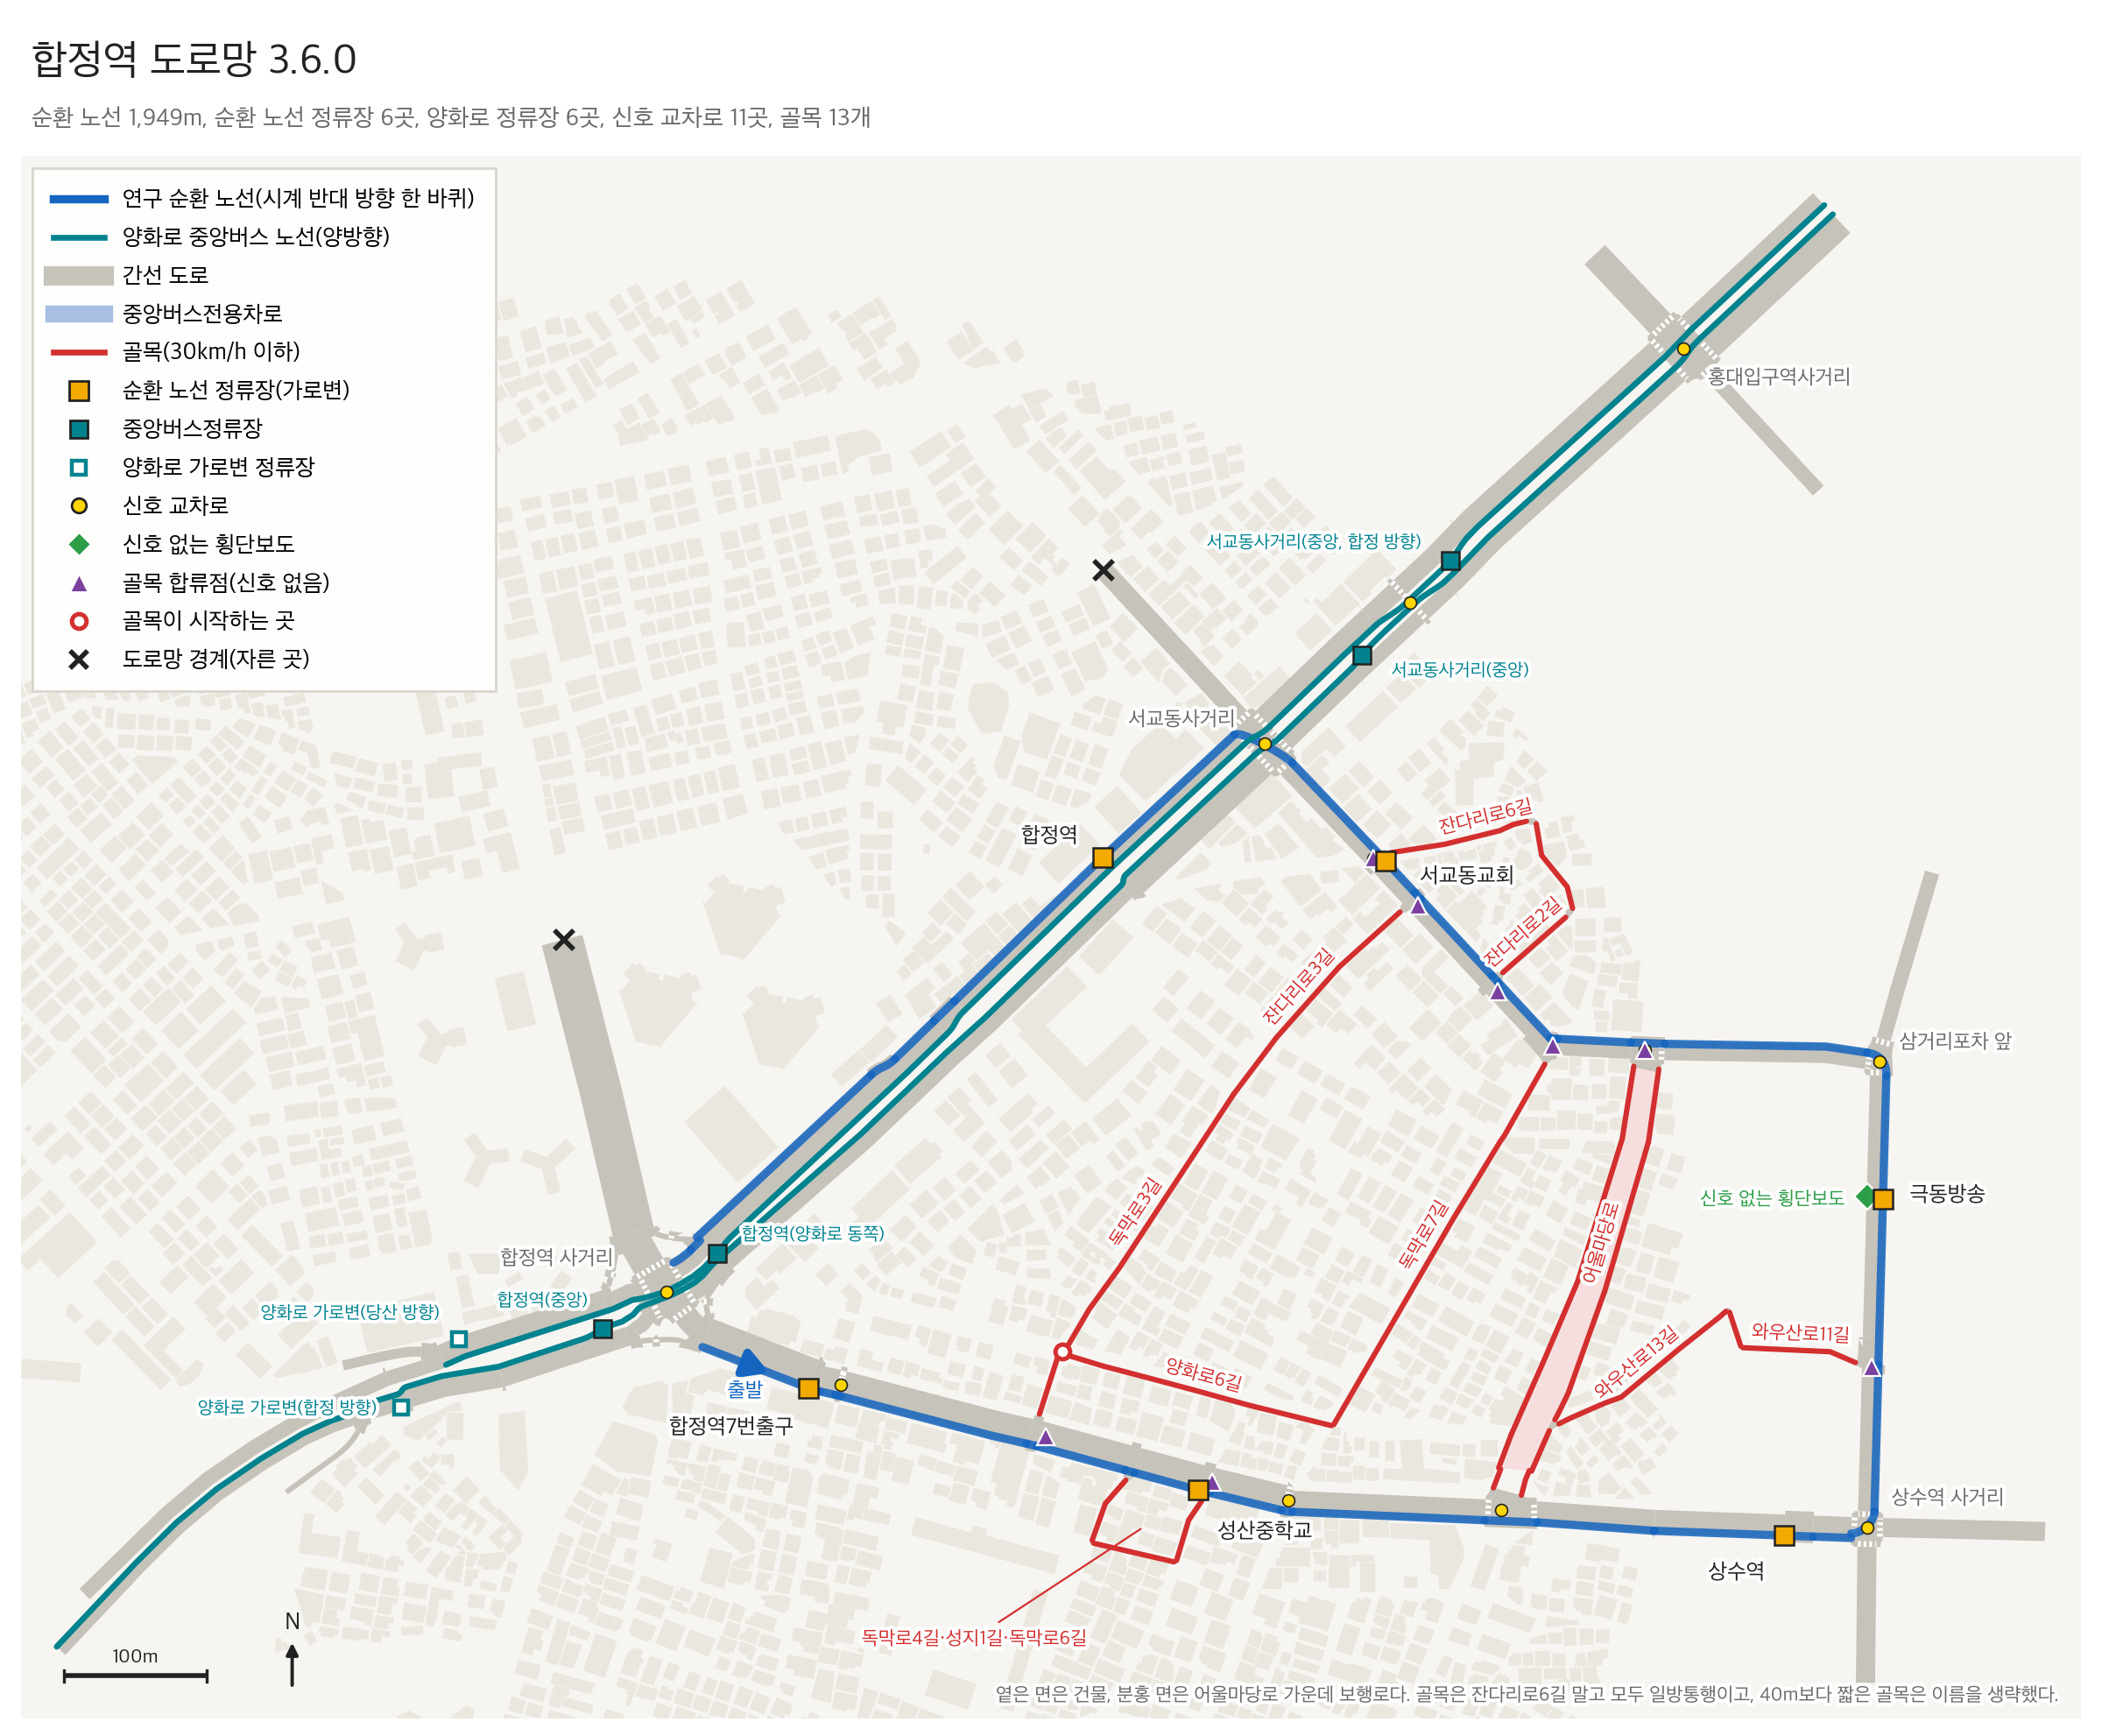
\includegraphics[width=\textwidth]{../../maps/hapjeong/references/hapjeong_map.png}\end{center}

\textbf{지도 보는 법.} 파란 선은 연구 버스 경로다. 빨간 선은 골목이다. 보라 세모는 골목 차가 버스 길로 나오는 곳이다. 청록 선과 네모는 양화로 중앙버스 노선과 정류장이다.

\newpage
\head{길마다 늘어나는 시나리오}
버스 160번 주행(혼잡한 교통)에서 쟀다. 앞 숫자는 그 길이 없을 때, 뒤 숫자는 지금이다. 길이 없으면 그 길에서 나온 차만큼 줄어든다고 보고 셌다.

\vspace{4pt}
\road{jandari6}{잔다리로6길}{46}{74}{205}{250}\hfill
\road{jandari3}{독막로3길 북쪽 + 잔다리로3길}{53}{74}{231}{250}

\vspace{8pt}
\road{dongmak6}{독막로6길 고리}{60}{74}{203}{250}\hfill
\road{wausan11}{와우산로11길 + 와우산로13길}{71}{74}{200}{250}

\vspace{8pt}
\road{jandari2}{잔다리로2길 + 잔다리로6길 남쪽}{71}{74}{225}{250}\hfill
\road{dongmak3}{독막로3길}{71}{74}{232}{250}

\vspace{8pt}
\road{eoulmadang}{어울마당로}{72}{74}{230}{250}\hfill
\road{dongmak7}{양화로6길 + 독막로7길}{74}{74}{225}{250}

\newpage
\head{어울마당로 연결과 신호}
\begin{itemize}
\item 어울마당로는 독막로 60m 앞에서 끊겨 있었다. 이번에 독막로까지 이었다.
\item 이었더니 버스가 한 바퀴에 17초 늦어졌다.
\item 원인은 신호다. 교차로 신호 주기가 90초에서 100초로 바뀌어, 다음 교차로(상수역 사거리)와 엇갈렸다.
\item 신호를 원래 90초로 고정했다. 버스 시간이 원래대로 돌아왔다.
\end{itemize}

{\begin{tabular}{@{}lrrr@{}}
\toprule
 & 잇기 전 & 잇기만 함 & 지금 \\
\midrule
버스 한 바퀴 시간 & 444초 & 461초 & 444초 \\
300번 중 사고·정체 & 11번 & 10번 & 6번 \\
버스 80번 중 완주 & 78, 79번 & 73, 76번 & 76, 79번 \\
\bottomrule
\end{tabular}}

\vspace{3pt}
완주는 교통이 다른 두 묶음의 결과다. 같은 도로도 묶음마다 1\textasciitilde{}2번씩 오르내린다.

\head{팀원별로 볼 것}
\begin{itemize}
\item \textbf{신호}: 독막로·어울마당로 교차로 신호를 \texttt{signals.add.xml}에 새로 적었다. 단계와 시간은 전과 같다.
\item \textbf{시나리오}: 끼어들기는 잔다리로6길, 잔다리로3길, 독막로6길 고리에서 주로 난다.
\item \textbf{대중교통}: 양화로 정류장과 중앙버스 노선은 그림에만 있다.
\end{itemize}
\end{document}
